\uuid{CPgC}
\chapitre{Courbes planes}
\sousChapitre{Courbes paramétrées}
\titre{Courbes paramétrées et chaînette}
\theme{courbes paramétrées}
\auteur{}
\datecreate{2023-03-01}
\organisation{AMSCC}
\contenu{

\begin{minipage}{0.49\textwidth}
	La chaînette est le nom que porte la courbe obtenue en tenant 
	une corde (ou un collier, un fil,\ldots) par deux extrémités.
	Voici l'équation cartésienne d'une chaînette :
	$$y = a \ch\left( \frac x a \right)$$  
	
	Le paramètre $a>0$ dépend de la chaînette : on peut écarter plus ou moins les mains.
Ou, ce qui revient au même, si l'on garde les mains fixes, on peut prendre des cordes de différentes longueurs.
	\end{minipage}
\hfill
	\begin{minipage}{0.5\textwidth}
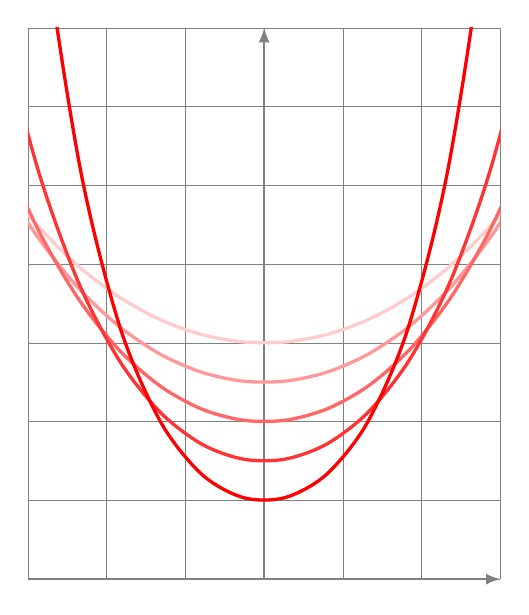
\begin{tikzpicture}
\def\xmin{-3}; 
\def\xmax{+3}; 
\def\ymin{0}; 
\def\ymax{+7};
\draw[help lines] (\xmin,\ymin) grid (\xmax,\ymax);
\clip (\xmin,\ymin-0.1) rectangle (\xmax,\ymax);
\draw[->,>=latex,thick,gray] (\xmin,0)--(\xmax,0);
\draw[->,>=latex,thick,gray] (0,\ymin)--(0,\ymax);
% \def\a{+1};
% \draw [thick, domain=\xmin:\xmax] plot(\x,{exp(\x)});
\foreach \a/\macoul in {3.0/20,2.5/40,2.0/60,1.5/80,1.0/100}{
	\draw [very thick, color=red!\macoul,samples=20,smooth] plot(\x,{\a*(exp(\x/\a)+exp(-\x/\a))/2});
}; 

% \draw [thick, color=blue] plot(\x,{(exp(\x)-exp(-\x))/2});
\end{tikzpicture}
	\end{minipage}
			
			
Le cosinus hyperbolique et le sinus hyperbolique sont la partie paire et impaire de l'exponentielle :
$$\ch(x) = \frac{e^x + e^{-x}}{2}, \qquad \sh(x) = \frac{e^x - e^{-x}}{2}.$$


\begin{center}
	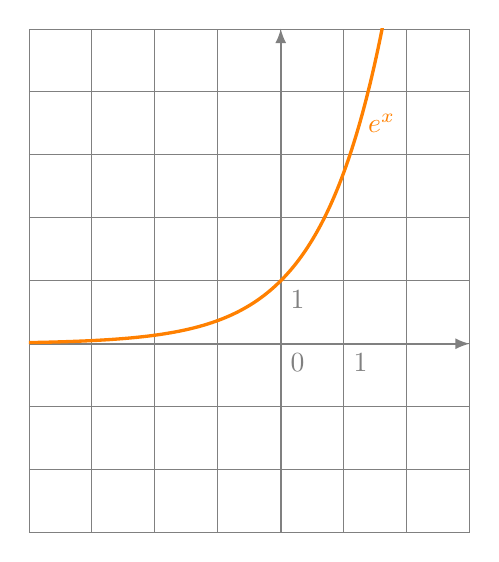
\begin{tikzpicture}[scale=0.8]
\def\xmin{-4}; 
\def\xmax{+3}; 
\def\ymin{-3}; 
\def\ymax{+5};

\draw[help lines] (\xmin,\ymin) grid (\xmax,\ymax);
\draw[->,>=latex,thick,gray] (\xmin,0) -- (\xmax,0);
\draw[->,>=latex,thick,gray] (0,\ymin) -- (0,\ymax);
\clip (\xmin,\ymin) rectangle (\xmax,\ymax);

%  \def\a{+1};
\draw [very thick, color=orange,samples=200,smooth] plot(\x,{exp(\x)});
\node[color=orange] at (1.6,3.5) {$e^x$};  
%  \draw [thick, color= red] plot(\x,{(exp(\x)+exp(-\x))/2});
%  \draw [thick, color=blue] plot(\x,{(exp(\x)-exp(-\x))/2});
\node[below right,gray] at (0,0) {$0$};
\node[below right,gray] at (1,0) {$1$};
\node[below right,gray] at (0,1) {$1$};
\end{tikzpicture}
	\qquad
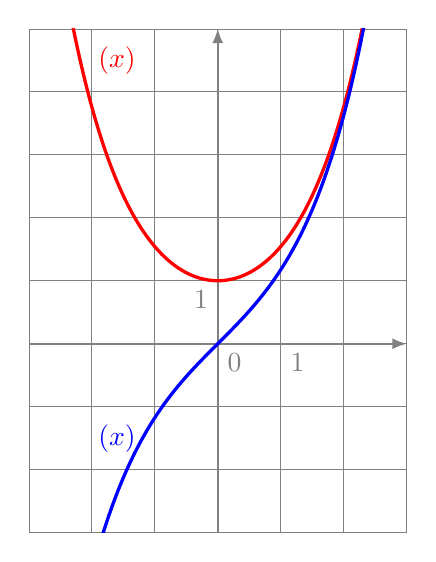
\begin{tikzpicture}[scale=0.8]
\def\xmin{-3}; 
\def\xmax{+3}; 
\def\ymin{-3}; 
\def\ymax{+5};
\draw[help lines] (\xmin,\ymin) grid (\xmax,\ymax);
\draw[->,>=latex,thick,gray] (\xmin,0)--(\xmax,0);
\draw[->,>=latex,thick,gray] (0,\ymin)--(0,\ymax);
\clip (\xmin,\ymin) rectangle (\xmax,\ymax);
\def\a{+1};
% \draw [thick, domain=\xmin:\xmax] plot(\x,{exp(\x)});
\draw [very thick, color=red,samples=200,smooth] plot(\x,{(exp(\x)+exp(-\x))/2});
% \beameronly{\uncover<5->}{
\draw [very thick, color=blue,samples=200,smooth] plot(\x,{(exp(\x)-exp(-\x))/2});
%};
\node[color=red] at (-1.6,4.5) {$\ch(x)$};  
%  \beameronly{\uncover<5->}{
\node[color=blue] at (-1.6,-1.5) {$\sh(x)$};  
%};
\node[below right,gray] at (0,0) {$0$};
\node[below right,gray] at (1,0) {$1$};
\node[below left,gray] at (0,1) {$1$};
\end{tikzpicture}
\end{center}
			

	

\begin{enumerate}
	\item \question{ Démontrer les propriété suivante : }
	\label{prop:chainette1}
	\begin{enumerate}
		\item $\ch^2(x) - \sh^2(x) = 1$, pour tout $x \in \R$.
		\reponse{$\ch^2 x- \sh^2 x = \frac14 \big[ (e^x+e^{-x})^2 - (e^x-e^{-x})^2 \big] = 
			\frac14 \big[ (e^{2x}+2+e^{-2x}) - (e^{2x}-2+e^{-2x})  \big] = 1$.}
		\item $\ch '(x) = \sh(x)$ et $\sh'(x) = \ch(x)$.
		\reponse{$\frac{d}{dx}(\ch x) = \frac{d}{dx} \frac{e^x+e^{-x}}{2} = \frac{e^x-e^{-x}}{2}  = \sh x$.}
	\end{enumerate}
   \item 	Les fonctions trigonométriques $\cos$ et $\sin$ sont dites << circulaires >>. On rappelle les formules d'Euler :
   $$\cos(x) = \frac{e^{\ii x} + e^{-\ii x}}{2}, \qquad \sin(x) = \frac{e^{\ii x} - e^{-\ii x}}{2\ii}.$$
   L'analogie avec la définition de $\ch(x)$ et $\sh(x)$ justifie les termes << cosinus >> et << sinus >>. 
   Reste à justifier le terme << hyperbolique >> :
   
   	On considère les courbes paramétrées $C_1 \colon \left\{
   	\begin{array}{l}
   	x(t) = \cos(t)\\
   	y(t) = \sin(t)
   	\end{array}
   	\right.$ et $C_2 \colon \left\{
   	\begin{array}{l}
   	x(t) = \ch(t)\\
   	y(t) = \sh(t)
   	\end{array}
   	\right.$
   	
   	\question{ Tracer des représentations graphiques de chacune de ces courbes paramétrées et commenter les calculs de $x(t)^2+y(t)^2$ et $x(t)^2 - y(t)^2$. }

   \reponse{Si on dessine une courbe paramétrée par $(x(t) = \cos t,y(t) = \sin t)$ alors
   	$x(t)^2+y(t)^2 = \cos^2 t + \sin^2 t =1$. Donc il s'agit d'un cercle
   	(d'où le terme <<circulaire>>). 
   	Par contre si on dessine une courbe paramétrée par $(x(t) = \ch t, y(t) = \sh t)$.
   	Alors $x(t)^2 - y(t)^2 = \ch^2 t - \sh^2 t = 1$.
   	C'est l'équation d'une branche d'hyperbole ! }
   \item 		\'Etant donné un arc paramétré $\begin{array}[t]{cccc}
   \mathcal{C} :&\mathcal ]a;b[ &\rightarrow&\Rr^2\\
   &t&\mapsto&(x(t),y(t))
   \end{array}$, sa longueur dans une base orthonormale est donnée par la quantité 
   $$L = \int_a^b \sqrt{x'(t)^2 + y'(t)^2} \dt$$
   
   	On considère une chaînette dont le point le plus bas est $(0,a)$ et dont les extrémités ont pour coordonnées $(\pm x_0,y_0)$. On s'intéresse à la longueur $\ell$ de la courbe entre le point le plus bas et une des extrémités. 

   	\begin{enumerate}
   		\item \question{ En utilisant l'équation cartésienne, écrire sous forme de courbe paramétrée la chaînette décrite ci-dessus. }
   		\reponse{On rappelle l'équation de la chaînette : $y(x) =a \ch \frac x a$. On en déduit une écriture paramétrique en posant $x(t)=t$ et $y(t) = a \ch \frac{x(t)}{a}$ pour tout $t \in [-x_0 ; x_0]$. }
   		\item \question{ Montrer que la demi longueur de la chaînette $\ell$ vaut $\ell=a\sh\left(\frac{x_0}{a}\right)$. }
   		\reponse{
   			Par définition, la demi longueur vaut
   			$$\ell = \int_0^{x_0} \sqrt{1+y'(x)^2} dx.$$
   			Ainsi :
   			$$\begin{array}{rcl}
   			\ell 
   			&=& \int_0^{x_0} \sqrt{1+\sh^2 \left( \tfrac x a \right)} dx \quad \text{ car } \ch' \tfrac x a = \frac 1 a \sh \tfrac x a \\
   			&=& \int_0^{x_0} \sqrt{\ch^2 \left(\tfrac x a\right)} dx   \quad \text{ car } 1+\sh^2 u = \ch^2 u \\
   			&=& \int_0^{x_0} \ch \tfrac x a dx =  \left[ a \sh\left(\tfrac x a\right) \right]_0^{x_0} \\
   			&=& a \sh \left(\tfrac{x_0}{a}\right). \\
   			\end{array}$$}
   	\end{enumerate}
   \item On peut démontrer les propriétés suivantes des fonctions hyperboliques : 

   	\begin{enumerate}
   		\item La fonction $x \mapsto \ch x$ est une bijection
   		de $[0,+\infty[$ dans $[1,+\infty[$. Sa bijection réciproque est 
   		notée $\Argch x$. Donc :
   		$$\ch\left(\Argch(x)\right) = x  \quad \forall x \in [1,+\infty[ 
   		\qquad\qquad  \Argch\left(\ch(x)\right) = x
   		\quad   \forall x \in [0,+\infty[$$
   		\reponse{\'Etudions la restriction de la fonction $\ch : [0,+\infty[ \to [1,+\infty[$.
   			\begin{itemize}
   				\item Comme $\ch' x = \sh x \ge 0$, pour $x\ge 0$, alors la restriction de la fonction $\ch$ est croissante.
   				Elle est même strictement croissante (la dérivée ne s'annule qu'en $0$).
   				
   				\item Comme $\ch 0 =1$, que $\ch x \to +\infty$ lorsque $x \to +\infty$,
   				alors par continuité et la stricte croissance, la restriction $\ch : [0,+\infty[ \to [1,+\infty[$
   				est une bijection.
   			\end{itemize}
   			Par définition, la bijection réciproque de cette restriction est $\Argch x : [1,+\infty[ \to [0,+\infty[$
   			et vérifie :
   			$$\Argch\big(\ch x\big) = x \qquad \text{ pour tout } x \in [0,+\infty[$$
   			$$\ch\big(\Argch x\big) = x \qquad \text{ pour tout } x \in [1,+\infty[.$$	}
   		\item La fonction $x \mapsto \sh x$ est une bijection
   		de $\Rr$ dans $\Rr$. Sa bijection réciproque est 
   		notée $\Argsh x$. Donc :
   		$$\sh\left(\Argsh(x)\right) = x  \qquad\qquad  \Argsh\left(\sh(x)\right) = x
   		\quad   \forall x \in \Rr$$
   		\item Les fonctions $x \mapsto \Argch(x)$ et $x \mapsto \Argsh(x)$
   		sont dérivables et 
   		$$\Argch'(x) = \frac{1}{\sqrt{x^2-1}} \qquad\qquad \Argsh'(x) = \frac{1}{\sqrt{x^2+1}}.$$
   		\reponse{Comme la fonction $x \mapsto \ch'x$  ne s'annule pas sur $]0,+\infty[$
   			alors la fonction $\Argch$ est dérivable sur $]1,+\infty[$.
   			On calcule la dérivée par dérivation de l'égalité $\ch(\Argch x) = x$ :
   			$$\Argch' x \cdot \sh(\Argch x) = 1$$
   			puis on utilise l'identité $\ch^2 u - \sh^2 u = 1$ avec $u = \Argch x$ :
   			$$\Argch' x = \frac{1}{\sh(\Argch x)} = \frac{1}{\sqrt{\ch^2(\Argch x)-1}}
   			= \frac{1}{\sqrt{x^2-1}}.$$  }
   		\item Pour tout $x \geq 1$ : $\Argch(x)  =  \ln\left( x+\sqrt{x^2-1} \right)$.
   		\reponse{ Notons $f(x)=\ln\big(x+ \sqrt{x^2-1}\big)$. 
   			$$f'(x) = \frac{1+\frac{x}{\sqrt{x^2-1}}}{x+ \sqrt{x^2-1}} = \frac{1}{\sqrt{x^2-1}} = \Argch' x.$$ 
   			Comme de plus $f(1)=\ln(1)=0$ et $\Argch(1) = 0$ (car $\ch(0) = 1$), on en déduit que pour tout
   			$x\in \Rr$, $f(x) = \Argch(x)$.
   		}
   		\item Pour tout $x \in \R$ : $\Argsh(x)  =  \ln\left( x+\sqrt{x^2+1} \right)$.
   		\reponse{ Notons $f(x)=\ln\big(x+ \sqrt{x^2+1}\big)$. 
   			$$f'(x) = \frac{1+\frac{x}{\sqrt{x^2+1}}}{x+ \sqrt{x^2+1}} = \frac{1}{\sqrt{x^2+1}} = \Argsh' x.$$ 
   			Comme de plus $f(0)=\ln(1)=0$ et $\Argsh 0 = 0$ (car $\sh 0 = 0$), on en déduit que pour tout
   			$x\in \Rr$, $f(x) = \Argsh x$.
   		}
   	\end{enumerate}
   	\question{ En utilisant les propriétés des fonctions hyperboliques et l'équation cartésienne d'une chaînette, démontrer qu'une équation paramétrique de la chaînette est :
   	$$\forall t>0 \colon \left\{
   	\begin{array}{rcl}
   	x(t) &=& a \ln t \\
   	y(t) &=& \frac a 2 \left(t+\frac 1 t\right)
   	\end{array}
   	\right.
   	$$    }
   \reponse{Nous connaissons l'équation cartésienne $y=a\ch \left(\frac x a\right)$,
   	qui est équivalente à $\Argch\left(\frac y a\right) = \frac x a$.
   	Utilisons la forme logarithmique de la fonction $\Argch$: 
   	$\Argch u = \ln \left( u + \sqrt{u^2-1} \right)$ (pour $u \ge 1$).
   	
   	Nous obtenons :
   	$$\ln \left( \frac y a + \sqrt{\left(\frac y a\right)^2-1} \right) = \frac x a.$$
   	
   	Nous cherchons maintenant une paramétrisation $(x(t),y(t))$ de la chaînette, 
   	posons $x(t) = a \ln(t)$ (ce qui est toujours possible car $\ln$ 
   	est une bijection de $]0,+\infty[$ dans $\Rr$).
   	Alors l'équation précédente conduit (après simplification des $\ln$) à :
   	$$\frac{y(t)}{a} + \sqrt{\left(\frac{y(t)}{a}\right)^2-1} = t,$$
   	ou encore 
   	$$\sqrt{\left(\frac{y(t)}{a}\right)^2-1} = t - \frac{y(t)}{a}$$
   	ce qui implique en élevant au carré :
   	$${\left(\frac{y(t)}{a}\right)^2-1} = t^2 + \left(\frac{y(t)}{a}\right)^2- 2t\frac{y(t)}{a}$$
   	d'où $\frac{y(t)}{a} = \frac{t^2+1}{2t}$,
   	et donc $y(t) = \frac a2 \left(t+\frac 1 t\right)$.}
\end{enumerate}}
